\documentclass[./main.tex]{subfiles}

\begin{document}

%%----------------------------------------------------
\begin{figure}[H]
\centering
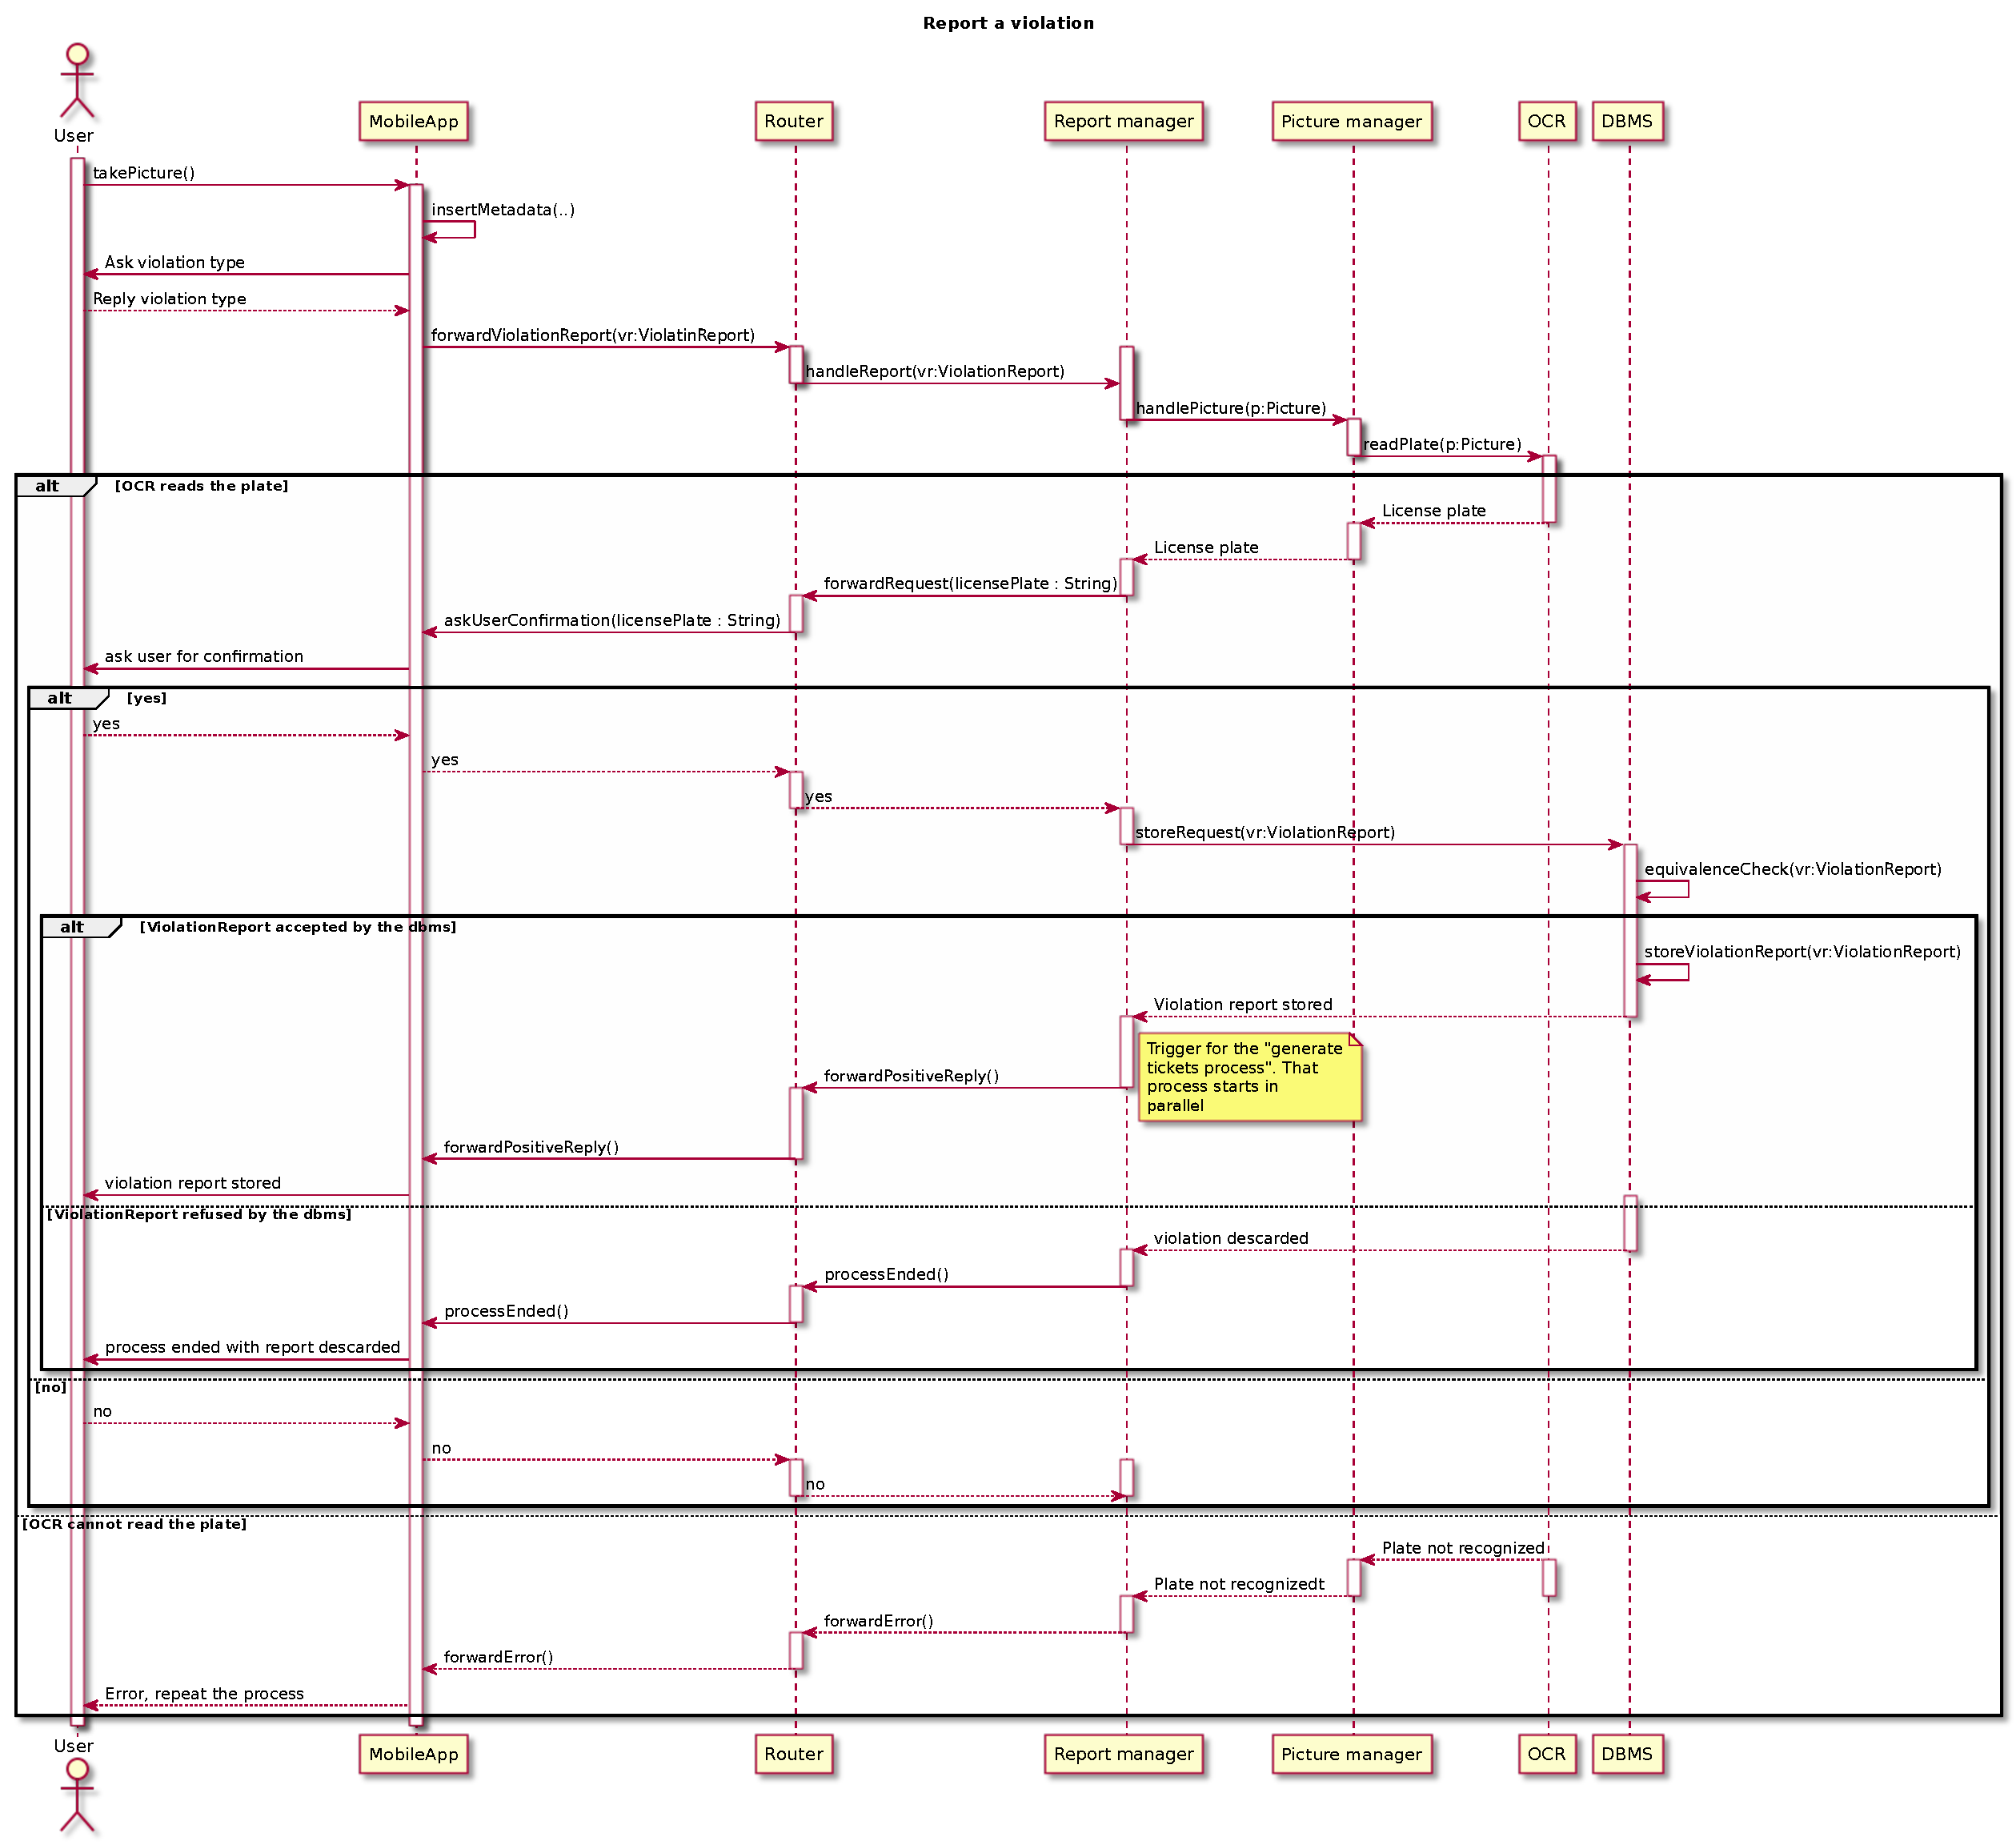
\includegraphics[width=\textwidth]{resources/sequence_diagrams/safereports}
\caption{Report a violation}
\end{figure}

%%-----------------------------------------------------
\begin{figure}[H]
\centering
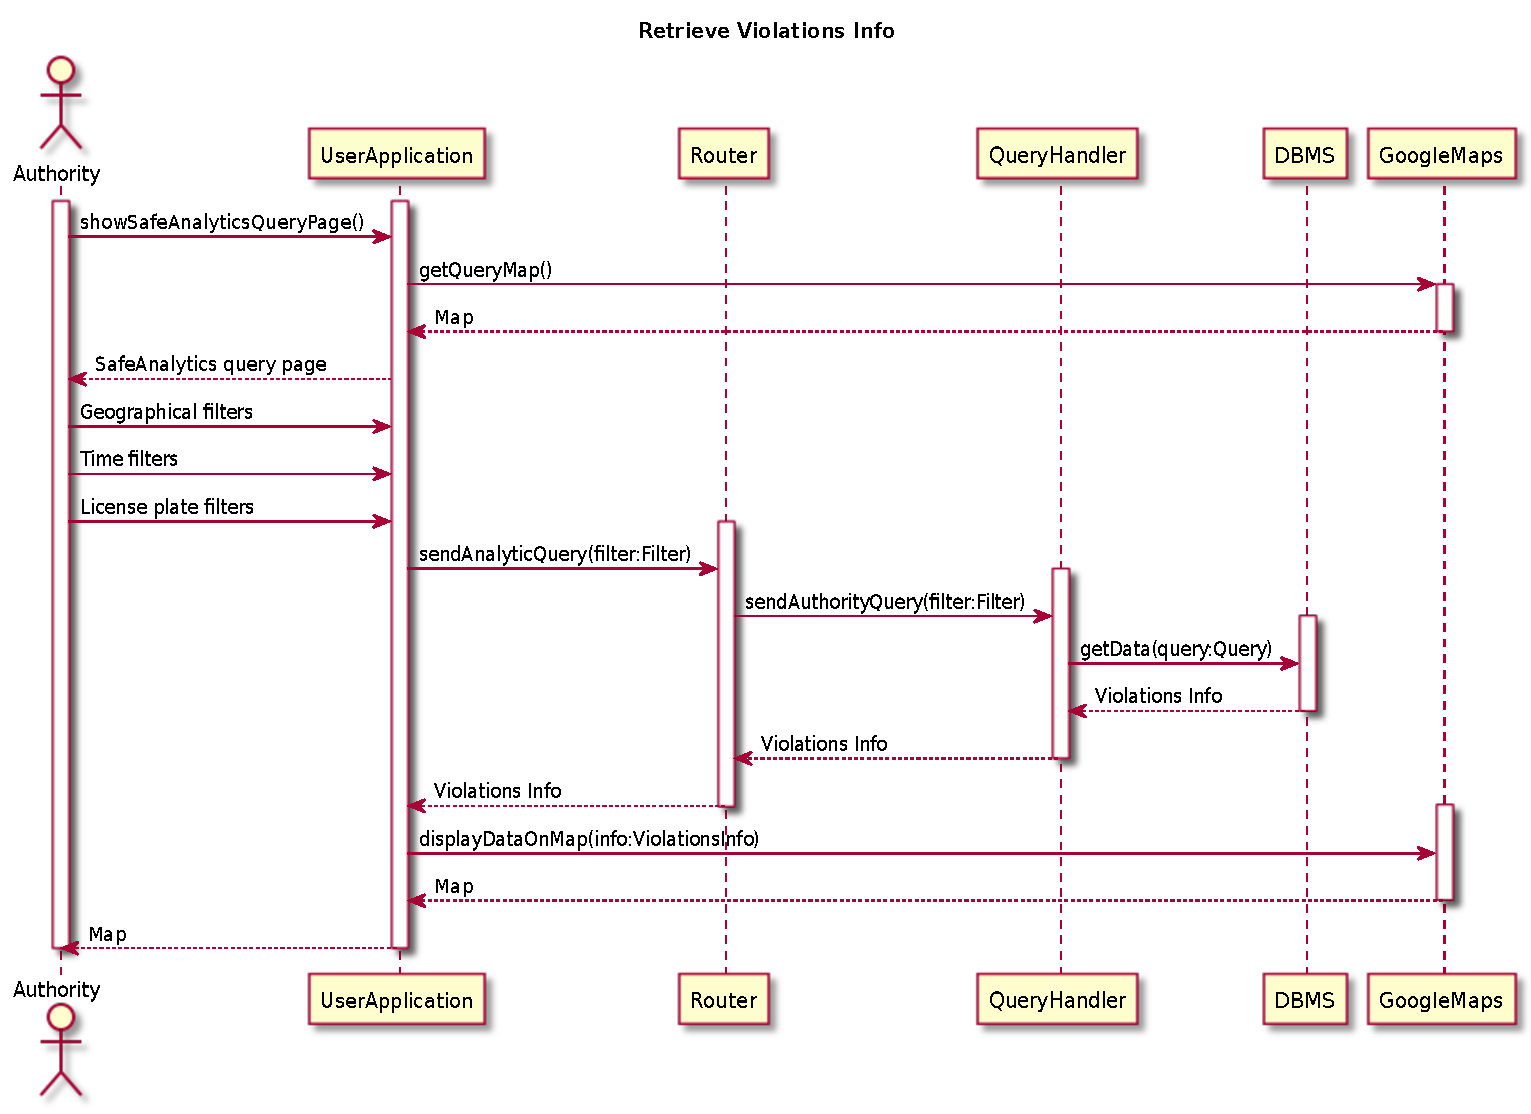
\includegraphics[width=\textwidth]{resources/sequence_diagrams/retrieve_violation_info}
\caption{Get information about reported violations}
\end{figure}

Here is shown how authorities get access to the information about the reported violations. This diagram is very similar to the one for the same functionality for the common user, so instead of representing it twice, the differences will be highlighted in this description.\\
The user is shown the SafeAnalytics main page, which consists in a query interface, changing according to the type of user. While common users are asked to insert position and time ranges, authorities can also ask for specific license plates. The selection of the position filter requires to display a map, so Google Maps is involved.\\
All the query data provided are stored in a Filter object and the query is passed to the DBMS, to retrieve the required data from the DB. This does not happen in a single step, as the request must pass through the Router and the QueryHandler. The response is sent back to UserApplication, which displays it on a map thanks again to Gooogle Maps.


%%-----------------------------------------------------
\begin{figure}[H]
\centering
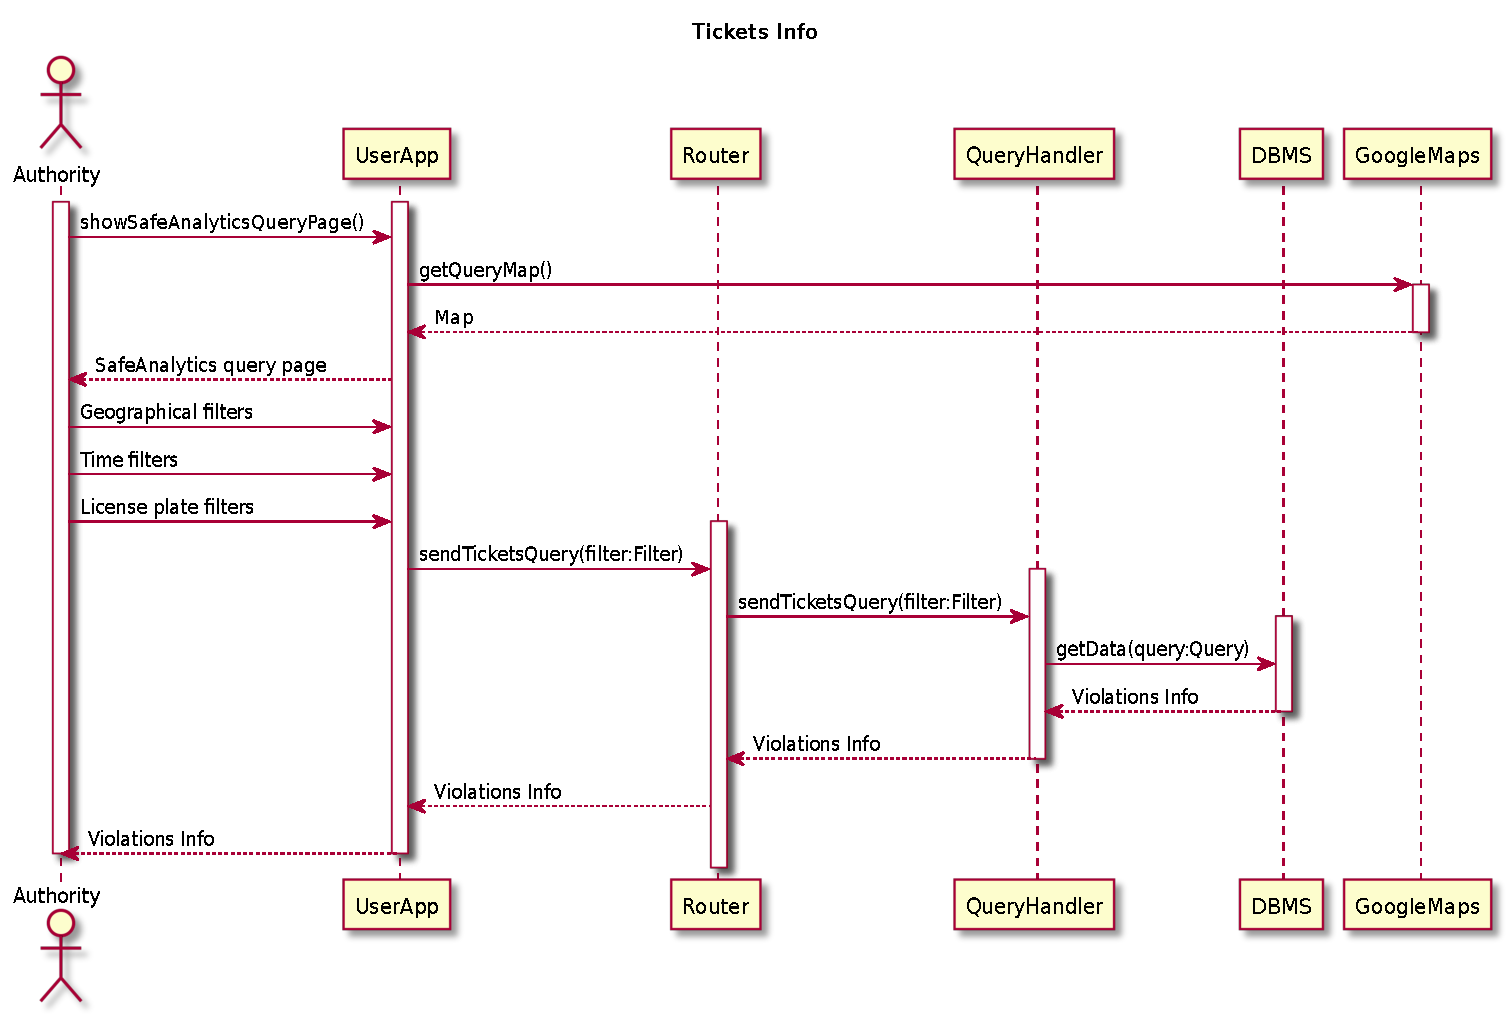
\includegraphics[width=\textwidth]{resources/sequence_diagrams/tickets_info}
\caption{Get information about generated tickets}
\end{figure}

Authorities get an interface similar to the one for getting information about the violations to get the tickets data. In the same way as for the other authority queries, a request for the information is forwarded to the DBMS. The statistics are not shown in a map (so Google Maps is not involved anymore), and the data flows back on the same path of the request to the user.

%%-----------------------------------------------------
\begin{figure}[H]
\centering
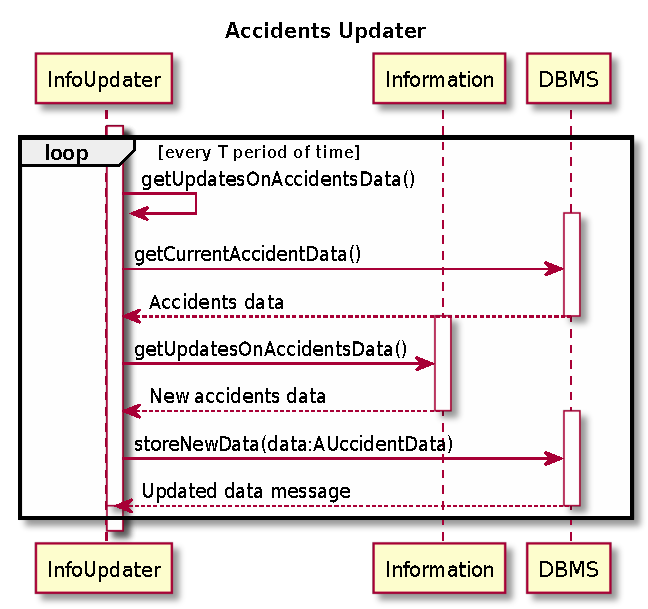
\includegraphics[width=\textwidth]{resources/sequence_diagrams/info_updater}
\caption{Update data from municipality}
\end{figure}

The system must periodically collect the accidents' data provided by the municipality. To do so, InfoUpdater contains a trigger to ask for new data. In order to not download the whole dataset provided by the municipality every time, a time stamp is saved to get the latest data only.

%%-----------------------------------------------------
\begin{figure}[H]
\centering
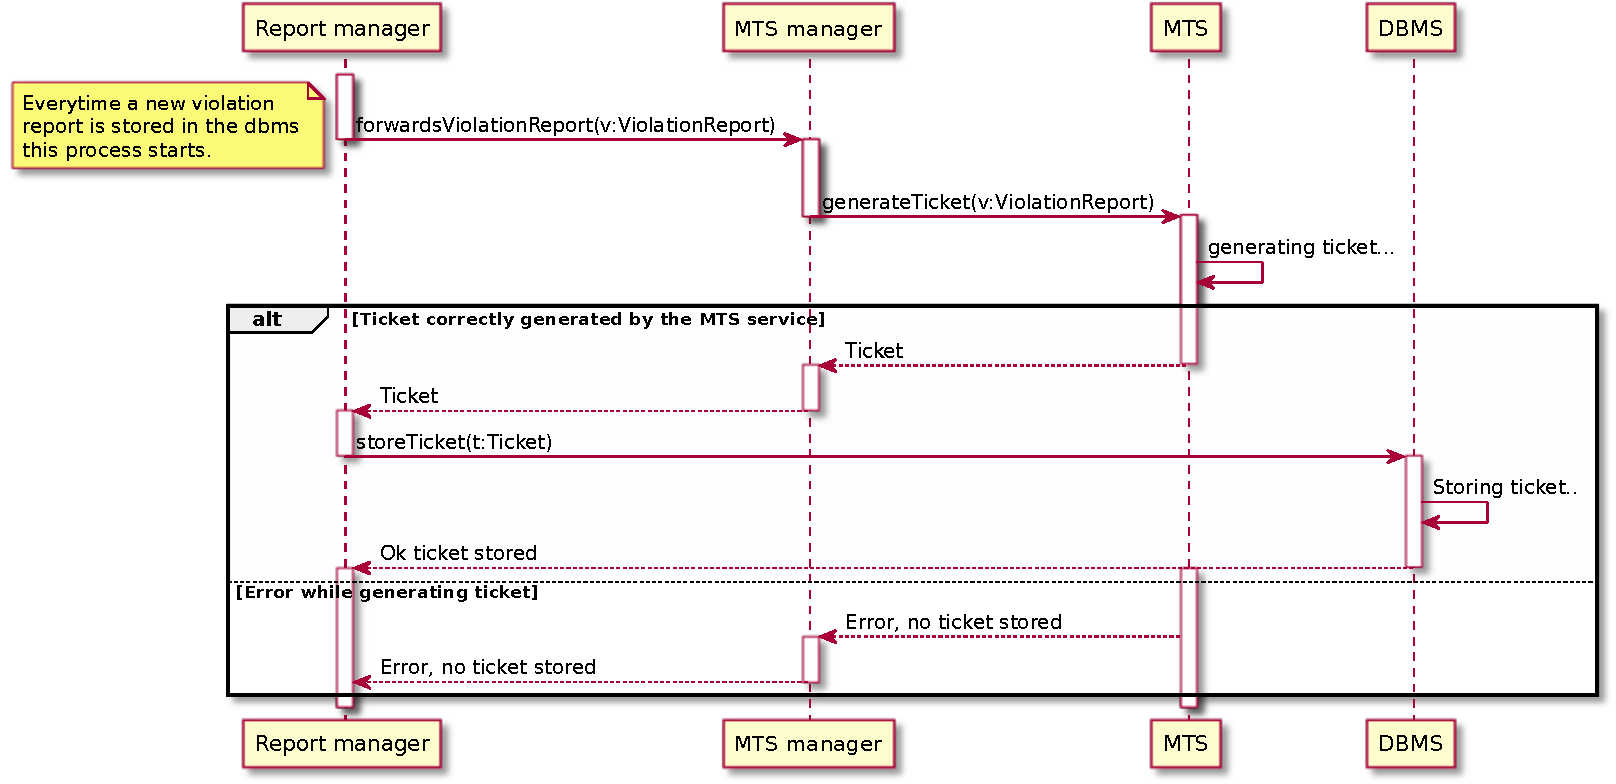
\includegraphics[width=\textwidth]{resources/sequence_diagrams/generate_tickets}
\caption{Generate tickets from reports}
\end{figure}

%%-----------------------------------------------------
\begin{figure}[H]
\centering
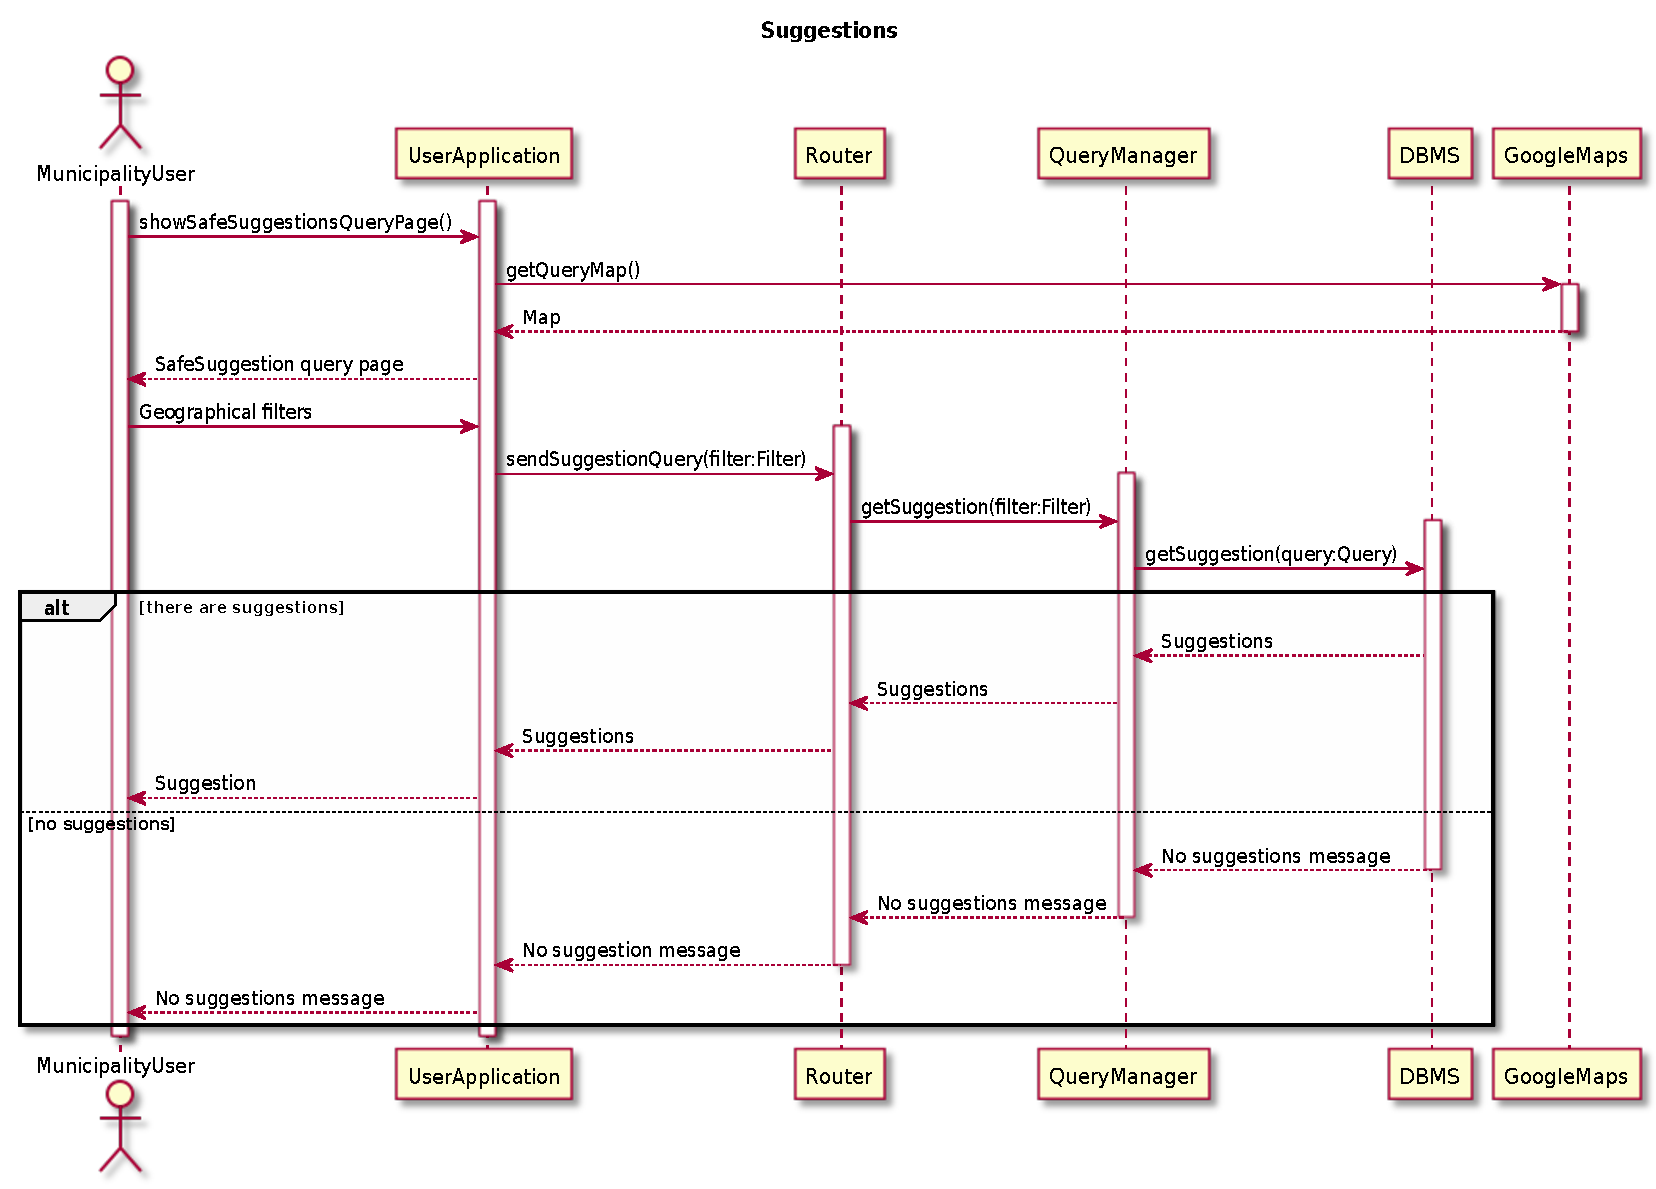
\includegraphics[width=\textwidth]{resources/sequence_diagrams/suggestions}
\caption{Get suggestions}
\end{figure}

%TODO maybe the data warehouse should be shown

The municipality user can get suggestions from a query page similar to the ones provided to the other users, but where the filters are only geographical. The DBMS gives an answer, which can be negative or a suggestion.

\end{document}